\begin{figure}
\begin{tabular}{@{}c@{}c@{}}
\begin{subfigure}[b]{0.5\textwidth}
\begin{center}
\begin{footnotesize}
\renewcommand{\arraystretch}{1.6}
\begin{tabular}{|ll|}
\hline
\multicolumn{2}{|c|}{\bf Points-to Invariants} \\
\hline
\hline
$\circled{\footnotesize J1} \  \cv{p} \pointsTo{} \{ \mlrf{\cpc{4}} \}$ & $\circled{\footnotesize J2} \  \mlrf{\cpc{4}} \pointsTo{} \{ \mlrs{\cpc{4}} \}$ \\
$\circled{\footnotesize J3} \  \cv{l} \pointsTo{} \{ \mlrs{\cpc{4}} \}$ & $\circled{\footnotesize J4} \  \mlrs{\cpc{4}} \pointsTo{} \{ \mlrs{\cpc{4}}, \heapr{} \}$ \\
$\circled{\footnotesize J5} \  \cv{i} \pointsTo{} \emptyset$            & $\circled{\footnotesize J6} \  \heapr{} \pointsTo{} \{ \mlrs{\cpc{4}}, \heapr{} \}$ \\
\hline
\end{tabular}
\end{footnotesize}
\end{center}
\caption{\label{fig:clistdeconspointstoinvs} Points-to Invariants at \cpc{5} of \cref{fig:llAllocCIR}}
\end{subfigure}%
&
\begin{subfigure}[b]{0.5\textwidth}
\begin{center}
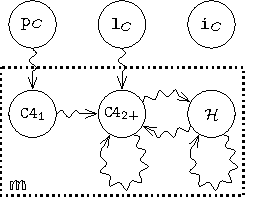
\includegraphics[scale=1]{chapters/figures/figClistDeconsCfgPointstoGraph.pdf}
\end{center}
\caption{\label{fig:clistdeconspointstograph} Points-to Graph at \cpc{5} of \cref{fig:llAllocCIR}}
\end{subfigure}%
\\
\end{tabular}
\caption{\label{fig:clistdeconspointstoinvsandgraph} Points-to Invariants and Points-to Graph at \cpc{5} of \cref{fig:llAllocCIR}}
\end{figure}